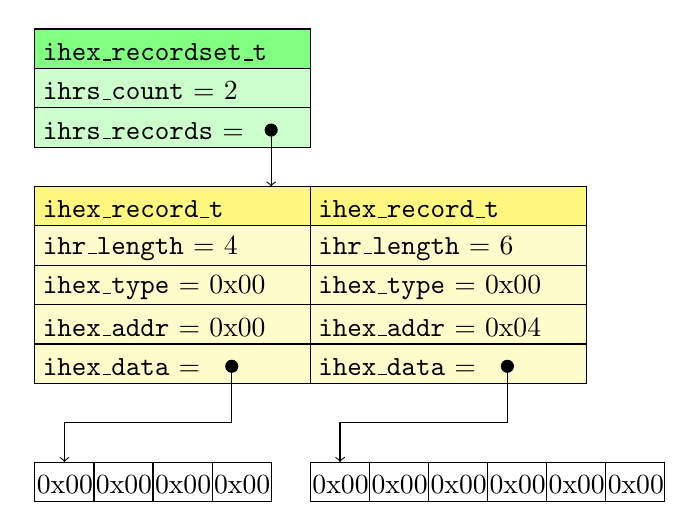
\begin{tikzpicture}
	\usetikzlibrary{arrows}
	\tikzstyle{attr}=[midway,text width=3.3cm,text height=0.3cm]
	\tikzstyle{green}=[fill=green!20]
	\tikzstyle{yellow}=[fill=yellow!20]	
			
	\draw [fill=green!50] (0,0) rectangle +(3.5,0.5) node [attr] {\texttt{ihex\_recordset\_t}};
	\draw [green] (0,-0.5) rectangle +(3.5,0.5) node [attr] {\texttt{ihrs\_count} = 2};
	\draw [green] (0,-1) rectangle +(3.5,0.5) node [attr] {\texttt{ihrs\_records} = };
			
	\draw [fill=yellow!50] (0,-2) rectangle +(3.5,0.5) node [attr] {\texttt{ihex\_record\_t}};
	\draw [yellow] (0,-2.5) rectangle +(3.5,0.5) node [attr] {\texttt{ihr\_length} = 4};
	\draw [yellow] (0,-3) rectangle +(3.5,0.5) node [attr] {\texttt{ihex\_type} = 0x00};
	\draw [yellow] (0,-3.5) rectangle +(3.5,0.5) node [attr] {\texttt{ihex\_addr} = 0x00};
	\draw [yellow] (0,-4) rectangle +(3.5,0.5) node [attr] {\texttt{ihex\_data} = };
			
	\draw [fill=yellow!50] (3.5,-2) rectangle +(3.5,0.5) node [attr] {\texttt{ihex\_record\_t}};
	\draw [yellow] (3.5,-2.5) rectangle +(3.5,0.5) node [attr] {\texttt{ihr\_length} = 6};
	\draw [yellow] (3.5,-3) rectangle +(3.5,0.5) node [attr] {\texttt{ihex\_type} = 0x00};
	\draw [yellow] (3.5,-3.5) rectangle +(3.5,0.5) node [attr] {\texttt{ihex\_addr} = 0x04};
	\draw [yellow] (3.5,-4) rectangle +(3.5,0.5) node [attr] {\texttt{ihex\_data} = };
			
	\draw[*->] (3,-0.7) -- (3,-1.5);
	\draw[*->] (2.5,-3.7) -- (2.5,-4.5) -- (0.75/2, -4.5) -- (0.75/2,-5);
	\draw[*->] (6,-3.7) -- (6,-4.5) -- (3.5+0.75/2, -4.5) -- (3.5+0.75/2,-5);
			
	\foreach \x in {0,0.75,1.5,2.25}{
		\draw (\x, -5.5) rectangle +(0.75,0.5) node [attr,text width=0.7cm] {0x00};
	};
			
	\foreach \x in {3.5,4.25,5,5.75,6.5,7.25}{
		\draw (\x, -5.5) rectangle +(0.75,0.5) node [attr,text width=0.7cm] {0x00};
	};
\end{tikzpicture}